\documentclass[a4j]{jarticle}
\usepackage[dvipdfmx]{graphicx}
\usepackage{amssymb}
\usepackage{subfigure}
\usepackage{here}

\begin{document}

\newcommand{\argmin}{\mathop{\rm arg~min}\limits}
\def \vector#1{\mbox{\boldmath $#1$}}
時系列モデルとして式 (\ref{garch1}) と式 (\ref{garch2}) で表される ARMA-GARCH(Autoregressive Moving Average - Generalized Autoregressive Conditional Heteroscedasticity)モデルを用いる.
\begin{equation}
y_t = \sum_{i=1}^p a_i y_{t-i} + \sum_{i=1}^q b_i \varepsilon_{t-i} + c + \varepsilon_{t} \hspace{1.5cm}\varepsilon_t \sim N(0,h_t) \hspace{0.5cm} i.i.d
\label{garch1}
\end{equation}
\begin{equation}
\displaystyle h_{t} = \omega + \sum_{i=1}^{r}\alpha_i\varepsilon_{t-i}^2 + \sum_{i=1}^{s}\beta_ih_{t-i}
\label{garch2}
\end{equation}

\section{クラスタ数の決定}
クラスタリングを行うにあたり,あらかじめクラスタ数を設定しておく必要がある.
ここでは,様々あるクラスタリング指標のうち,PseudoF と金尻先輩がこれに改良を加えた二つの合わせて三つのうちどの指標を用いるのか,またその指標のもと定まる最適クラスタ数を求める.

クラスタリング手法は階層的クラスタリングを用い,距離関数をユークリッド距離,クラスタ融合手法をウォード法とした.

クラスタリングにおける要素集合 $C$ の代表点には式 (\ref{medoid}) で表されるメドイドを用いる.
dist(\vector{x},\vector{y}) は要素 \vector{x} と \vector{y} との間のユークリッド距離であり,要素 $\vector{x} = [w_{x1},w_{x2},...,w_{xn}]$ として,式 (\ref{euqlidean}) で表される.
\begin{equation}
(メドイド) = \argmin_{\vector{x} \in C} \sum_{\vector{y} \in C - \{\vector{x}\}} dist(\vector{x},\vector{y})
\label{medoid}
\end{equation}
\begin{equation}
dist(\vector{x},\vector{y})  = \sqrt{ \sum^n_{i=1} ( w_{xi} - w_{yi} )^2}
\label{euqlidean}
\end{equation}

PseudoF は式 (\ref{PseudoF}) で表されるように重み付きクラスタ間普遍分散をクラスタ内分散で除したものとなっており,この値が大きいほどクラスタ間は疎でクラスタ内は蜜であることを意味する.
一般的にクラスタ間は疎でクラスタ内は蜜となったクラスタリング結果は良いものとされるので,PseudoF 値を大きくするようなクラスタ数を設定する.

\begin{equation}
\textrm{PseudoF} = \frac{\frac{1}{k-1} \displaystyle \sum^k_{i=1} n_{i}\hspace{0.1cm} dist(\vector{m_{i}},\vector{m})^2}{\frac{1}{N-k} \displaystyle \sum^k_{i=1}\displaystyle \sum_{\vector{x} \in C_i - \{\vector{m_i}\}} dist(\vector{x},\vector{m_{i}})^2}
\label{PseudoF}
\end{equation}
$k$ はクラスタ数とし,各クラスタ集合を $C_1,C_2,...,C_k$ と表す.
$n_i$ はクラスタ $C_i$ に属する要素数であり,$N$ は全要素数である.
また,$\vector{m_i}$ はクラスタ $C_i$ のメドイドであり,$\vector{m}$ は全要素に対するメドイドである.
Pseudo with Min は,クラスタ間のばらつき具合ををクラスタ間の距離を用いて定めるも用いる.
また,分母の小ささが全体の値の大きさに決定的な影響を与えないように分母部分に 1 を加算している.
\begin{equation}
\textrm{PseudoF with Mean} = \frac{\frac{1}{k} \displaystyle \sum^k_{i=1}\displaystyle \sum^k_{j=1} n_{i}\hspace{0.1cm} dist(\vector{m_{i}},\vector{m_j})^2}{1 + \displaystyle \sum^k_{i=1}\displaystyle \sum_{\vector{x} \in C_i - \{\vector{m_i}\}} dist(\vector{x},\vector{m_{i}})^2}
\label{PseudoFwithMean}
\end{equation}
\begin{equation}
\textrm{PseudoF with Min} = \frac{ \displaystyle \sum^k_{i=1} n_{i}\hspace{0.1cm} \min \{ dist(\vector{m_{i}},\vector{m_j}),j \neq i \}^2}{1 + \displaystyle \sum^k_{i=1}\displaystyle \sum_{\vector{x} \in C_i - \{\vector{m_i}\}} dist(\vector{x},\vector{m_{i}})^2}
\label{PseudoFwithMin}
\end{equation}

\newpage
\subsection{実測値に対して}
実測値に対してこれら三つの指標を用いた結果は図 \ref{normPseudoF} となった.
縦軸に指標の値をとり,横軸をクラスタ数とした.
表 \ref{normPseudoFresult} は各指標から定まる最適クラスタ数をまとめたものであり,図 \ref{normPseudoFresultPlot} はそれらの最適クラスタ数でクラスタリングを行ったときの主成分散布図である.

\begin{figure}[tb]
\begin{center}
\subfigure[PseudoF]{
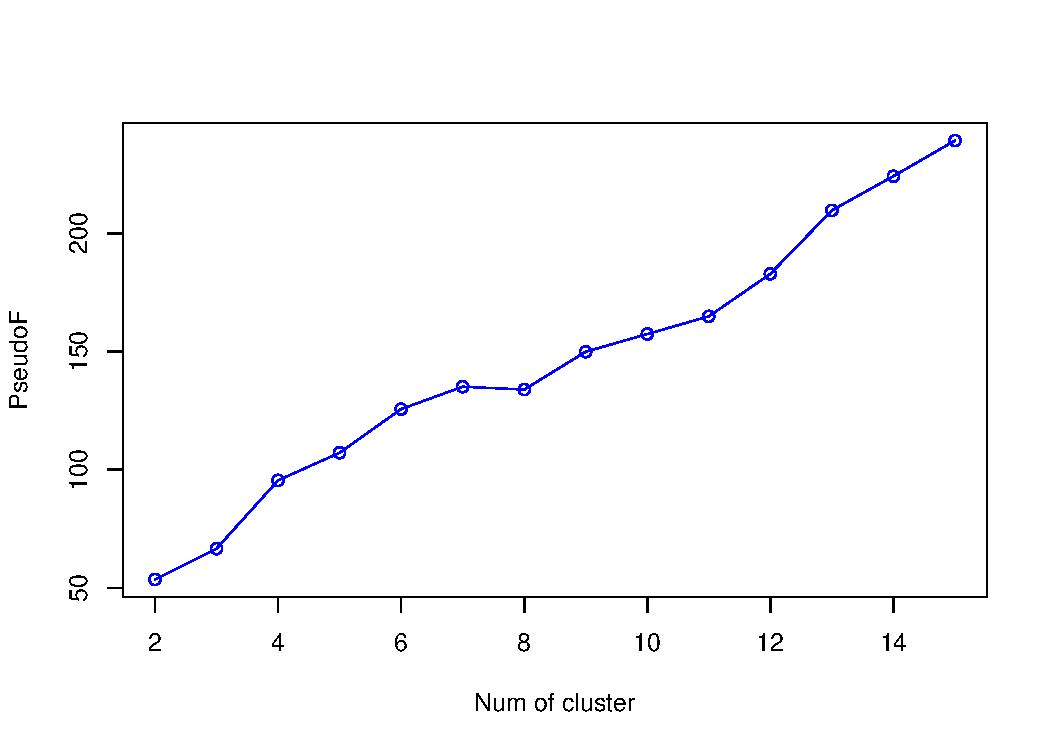
\includegraphics[width=0.33\hsize]{norm-PseudoF.pdf}
}~
\subfigure[PseudoF with Mean]{
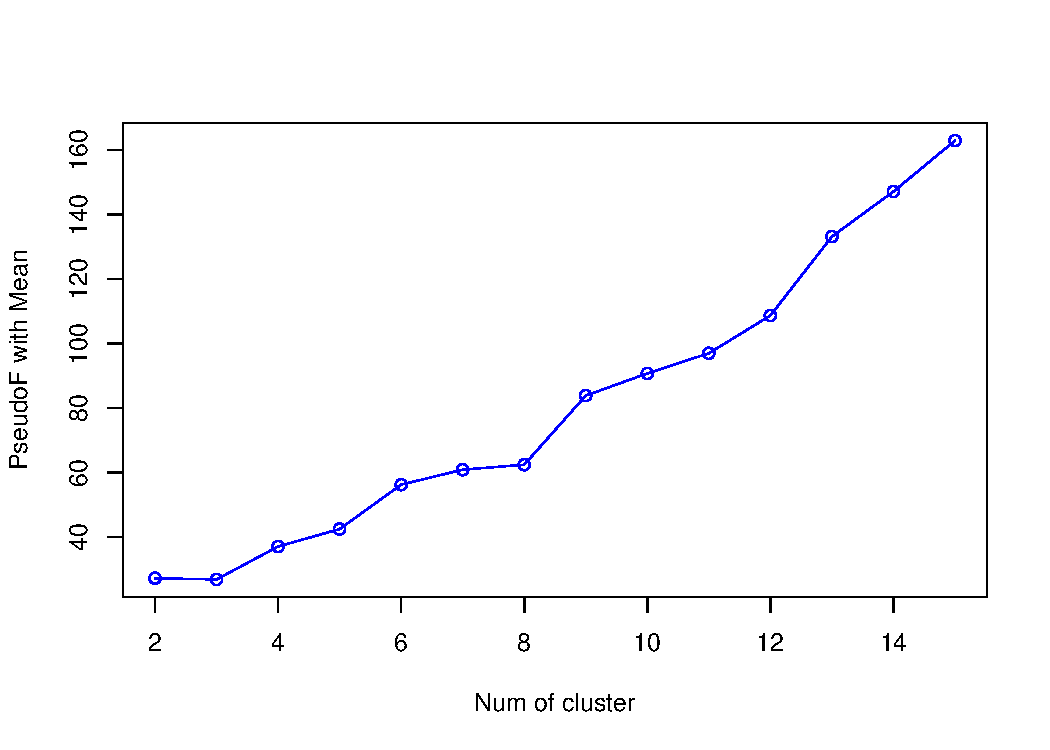
\includegraphics[width=0.33\hsize]{norm-PseudoFwithMean.pdf}
}~
\subfigure[PseudoF with Min]{
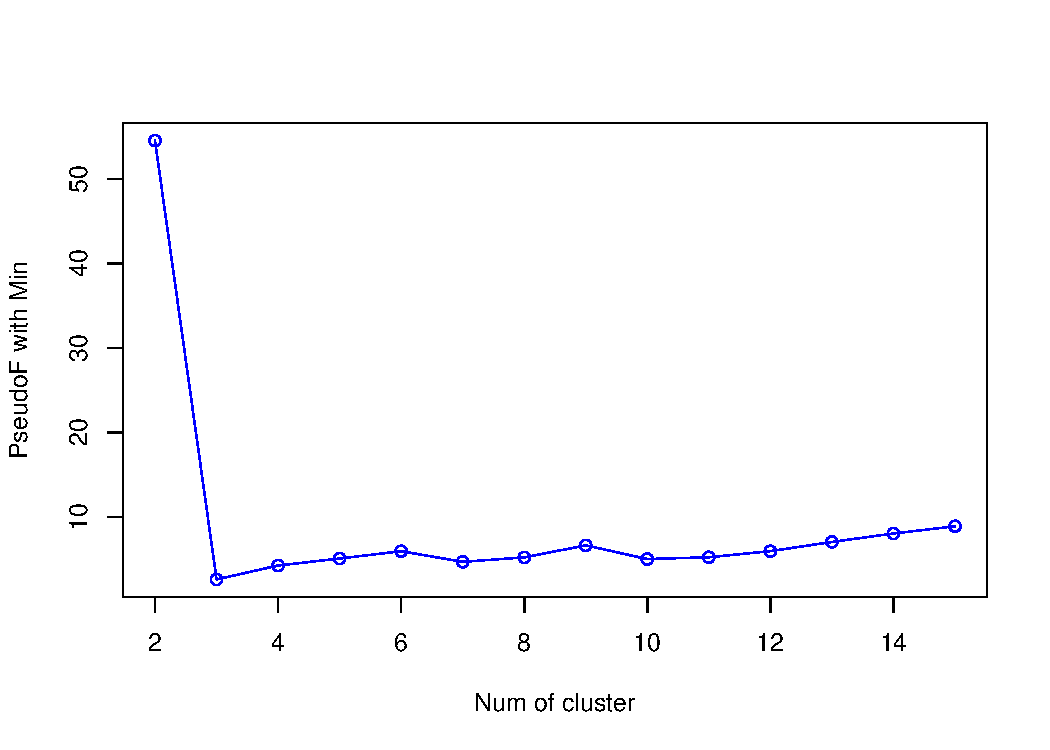
\includegraphics[width=0.33\hsize]{norm-PseudoFwithMin.pdf}
}
\caption{実測値における最適クラスタ数指標}
\label{normPseudoF}
\end{center}
\end{figure}

\begin{table}[tb]
\centering
\caption{実測値における最適クラスタ数}
\label{normPseudoFresult}
\begin{tabular}{|c|c|}
\hline
指標&最適クラスタ数\\
\hline
PseudoF&15\\
\hline
PseudoF with Mean&15\\
\hline
PseudoF with Min&2\\
\hline
\end{tabular}
\end{table}

\begin{figure}[tb]
\begin{center}
\subfigure[クラスタ数 2]{
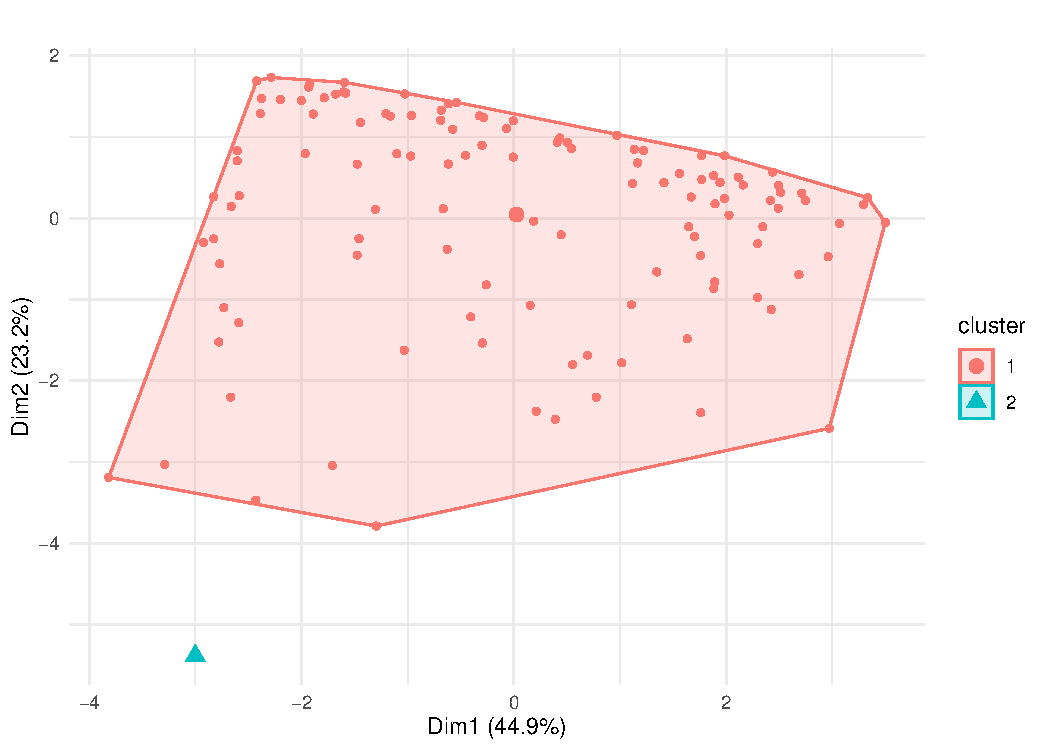
\includegraphics[width=0.5\hsize]{norm-compscatter-2.pdf}
}~
\subfigure[クラスタ数 15]{
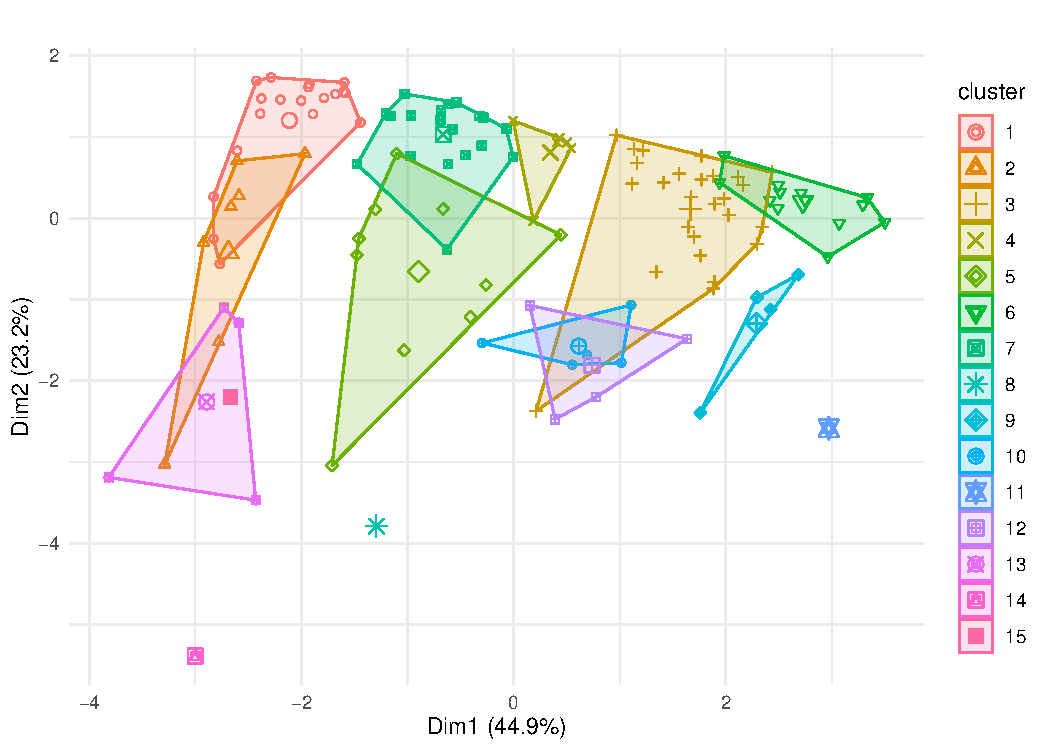
\includegraphics[width=0.5\hsize]{norm-compscatter-15.pdf}
}
\caption{実測値におけるクラスタリング結果の主成分散布図}
\label{normPseudoFresultPlot}
\end{center}
\end{figure}

図 \ref{normPseudoF}(a),図 \ref{normPseudoF}(b) の指標値は単調に増加しており,クラスタ数が 2 から 15 までの範囲では最適クラスタ数は 15 となった.
図 \ref{normPseudoF}(c) の指標値はクラスタ数 2 の場合に突出して大きくなっており,最適クラスタ数は 2 となった.

このような結果となるのは,クラスタ数 2 の時に形成される二つのクラスタ間は大きく離れているのだが,クラスタ数を増やすにつれてこれらのクラスタから分離して形成される新たなクラスタは,全要素に対するメドイドや分離前に属していなかったクラスタからは離れているものの,分離前に属していたクラスタからは近いためだと思われる.
したがって,クラスタ数 3 以上においてはクラスタの細分化が起こっていると考えられ,必要以上の細分化は一つのクラスタ内で完結した共通の特徴を損なわせるため生じないほうが良いという観点では,指標 PseudoF with Min が良いように思われる.

図 \ref{normPseudoFresultPlot}(a) より,クラスタ数 2 において形成される二つのクラスタのうち一方は要素数が 1 でもう一方のクラスタからは大きく離れた分布に位置していた.
この要素は 3/15(日)7:00-8:00 における計測データであった.
この計測データに対する ARMA-GARCH(2,2,1,1) による回帰結果は図 \ref{0315_07-reg} となっており,その回帰におけるパラメータは表 \ref{0315_07-param} となっていた.
比較のため 3/22(日)7:00-8:00 の計測データに対するものを載せている.
図 \ref{0315_07-reg} と表 \ref{0315_07-param} から,3/15(日)7:00-8:00 における回帰では,約 400ms のスパイク的な応答遅延が発生しておりこれは他のスパイク的な応答遅延が約 200ms であることと比べても大きな値である.
これにより,ノイズ項が従う正規分布の分散の回帰における定数項 $\omega$ の値が異常に大きくなりすぎていることが読み取れる.
この大きな 400ms 程度の遅延はほとんど起こらないものの異常ではないと考えられるため,回帰を行うにあたり,スパイク的な応答遅延を除くもしくは何らかの上限値を設けて置換するなどが必要かもしれない.
もしくは,標準化を行うなどして,ある一つのパラメータの大きさがクラスタリングにおける距離関数にて決定的な影響を与えないようにする必要があるだろう.

\begin{figure}[tb]
\begin{center}
\subfigure[3/15(日)7:00-8:00]{
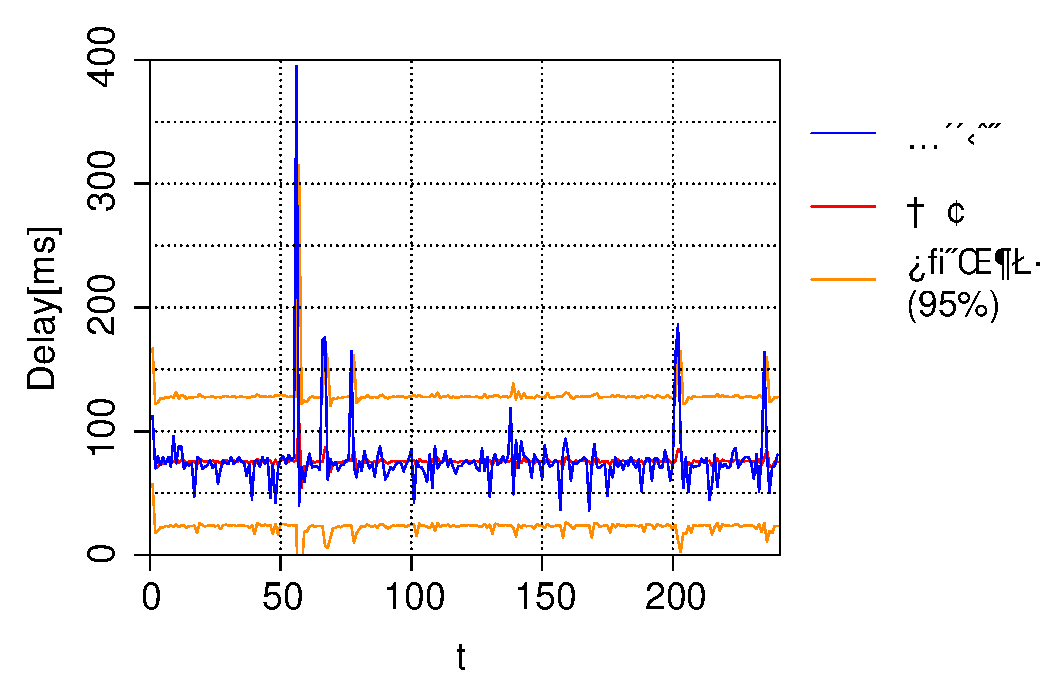
\includegraphics[width=0.5\hsize]{0315_07-plot.pdf}
}~
\subfigure[3/22(日)7:00-8:00]{
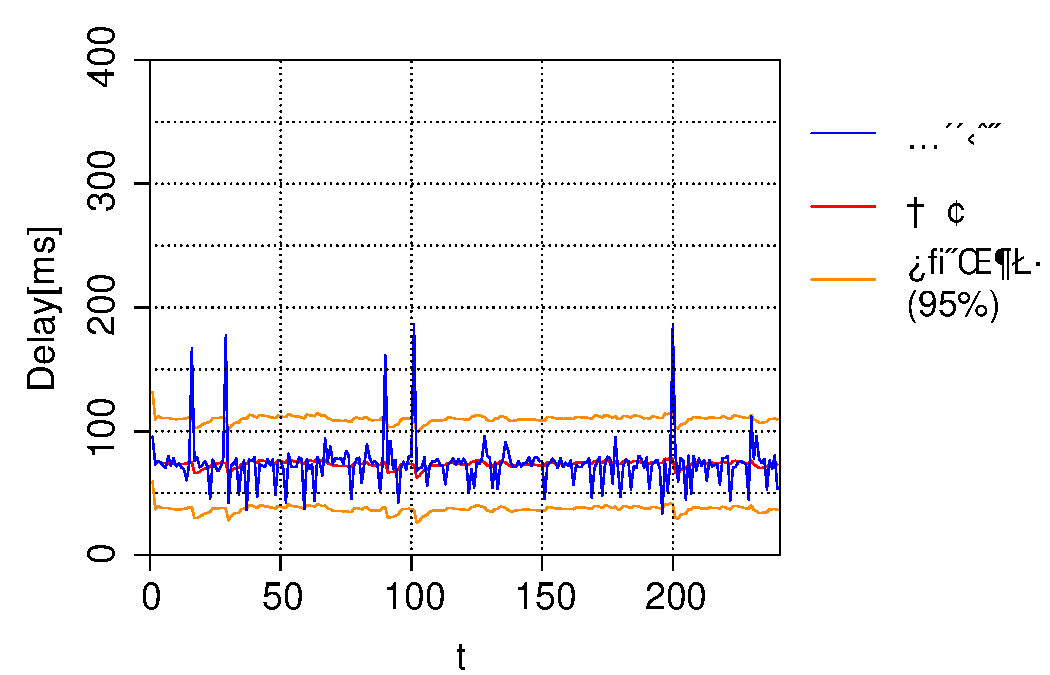
\includegraphics[width=0.5\hsize]{0322_07-plot.pdf}
}
\caption{実測値に対する ARMA-GARCH(2,2,1,1) での回帰結果}
\label{0315_07-reg}
\end{center}
\end{figure}

\begin{table}[tb]
\centering
\caption{回帰結果におけるパラメータ}
\label{0315_07-param}
\begin{tabular}{|c|c|c|}
\hline
&3/15(日)7:00-8:00&3/22(日)7:00-8:00\\
\hline
$c$&37.37&26.86\\
\hline
$a_1$&0.5457&0.5265\\
\hline
$a_2$&-0.0392&0.1082\\
\hline
$b_1$&-0.4351&-0.6159\\
\hline
$b_2$&-0.0635&-0.1387\\
\hline
$\omega$&703.18&55.78\\
\hline
$\alpha_1$&0.0995&$\ll0.0001$\\
\hline
$\beta_1$&$\ll0.0001$&0.8390\\
\hline
\end{tabular}
\end{table}

\newpage
\subsection{変動値に対して}
変動値に対してこれら三つの指標を用いた結果は図 \ref{diffPseudoF} となった.
表 \ref{diffPseudoFresult} は各指標から定まる最適クラスタ数をまとめたものであり,図 \ref{diffPseudoFresultPlot} はそれらの最適クラスタ数でクラスタリングを行ったときの主成分散布図である.

\begin{figure}[tb]
\begin{center}
\subfigure[PseudoF]{
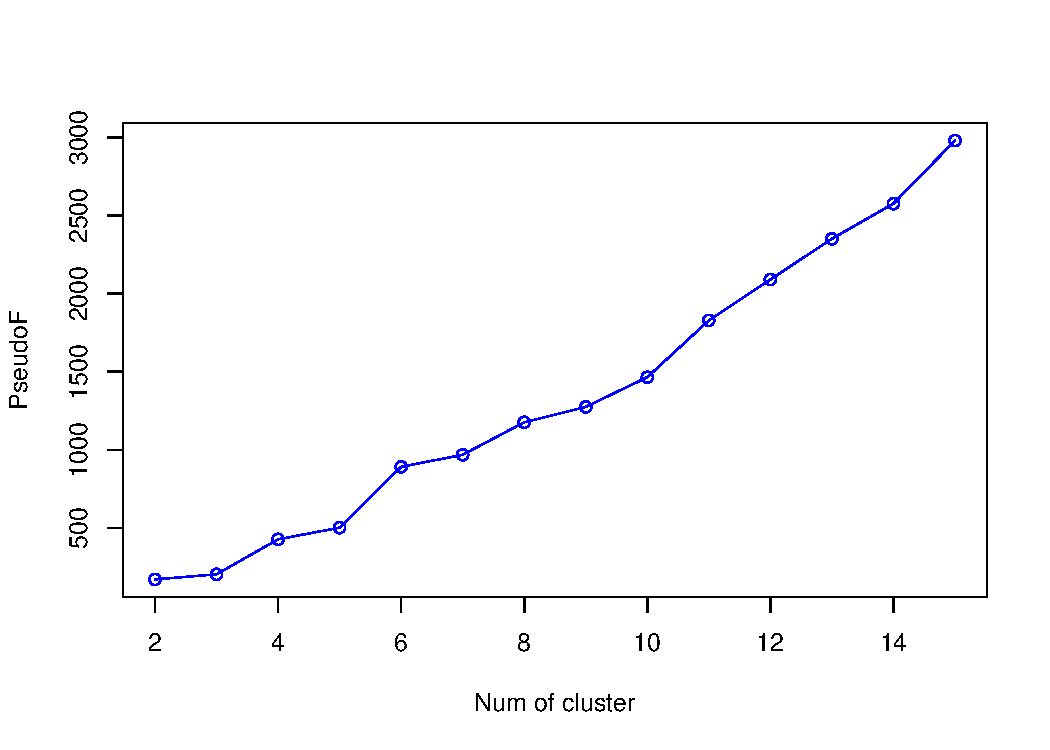
\includegraphics[width=0.33\hsize]{diff-PseudoF.pdf}
}~
\subfigure[PseudoF with Mean]{
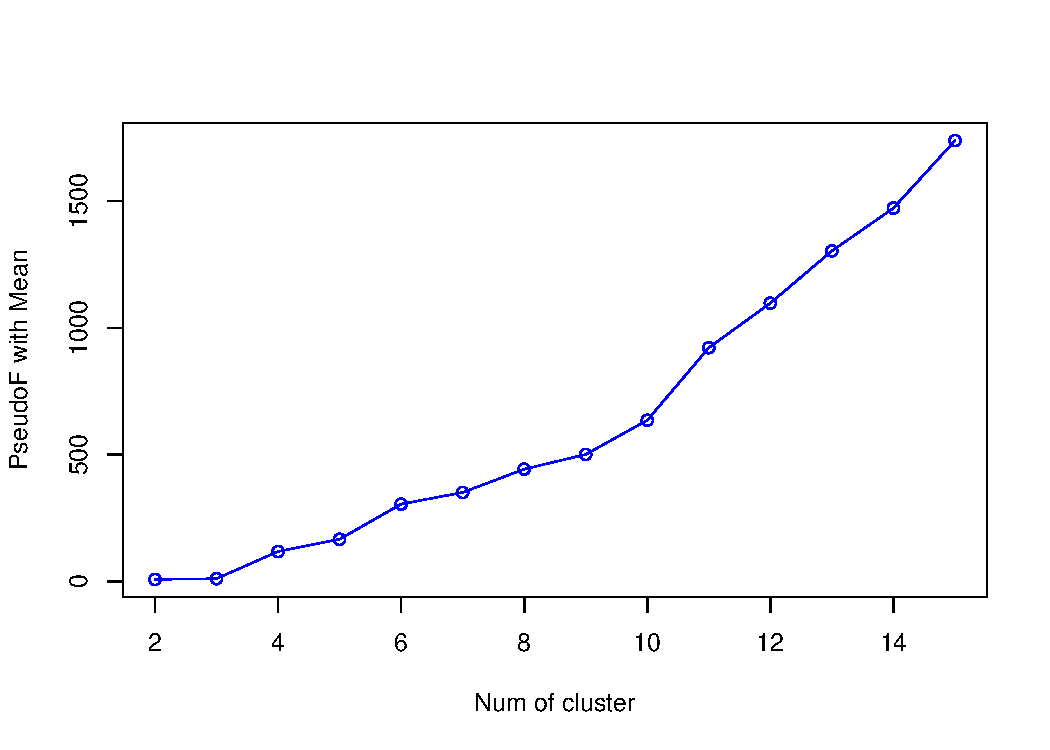
\includegraphics[width=0.33\hsize]{diff-PseudoFwithMean.pdf}
}~
\subfigure[PseudoF with Min]{
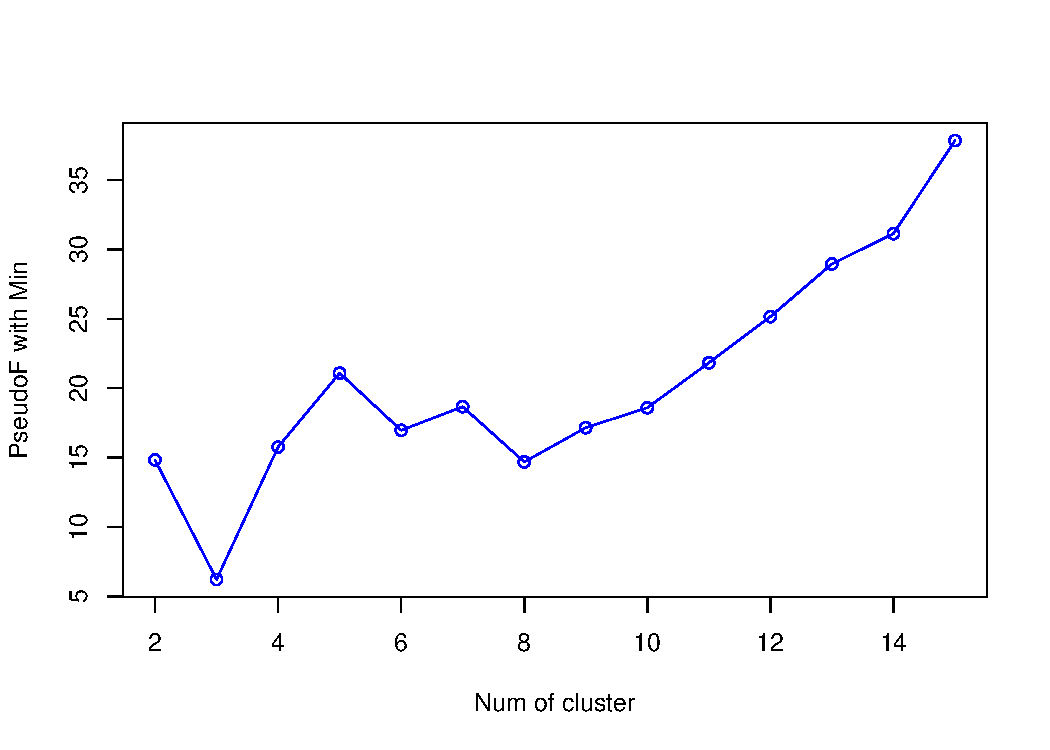
\includegraphics[width=0.33\hsize]{diff-PseudoFwithMin.pdf}
}
\caption{変動値における最適クラスタ数指標}
\label{diffPseudoF}
\end{center}
\end{figure}

\begin{table}[tb]
\centering
\caption{変動値における最適クラスタ数}
\label{diffPseudoFresult}
\begin{tabular}{|c|c|}
\hline
指標&最適クラスタ数\\
\hline
PseudoF&15\\
\hline
PseudoF with Mean&15\\
\hline
PseudoF with Min&5,15\\
\hline
\end{tabular}
\end{table}

\begin{figure}[tb]
\begin{center}
\subfigure[クラスタ数 5]{
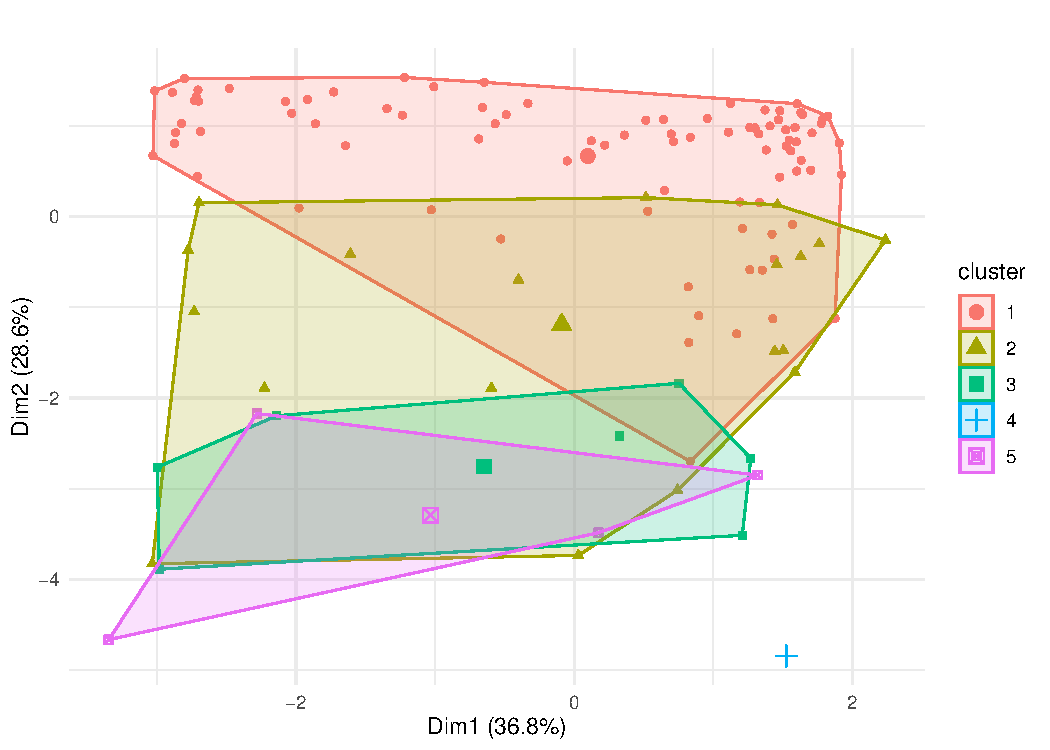
\includegraphics[width=0.5\hsize]{diff-compscatter-5.pdf}
}~
\subfigure[クラスタ数 15]{
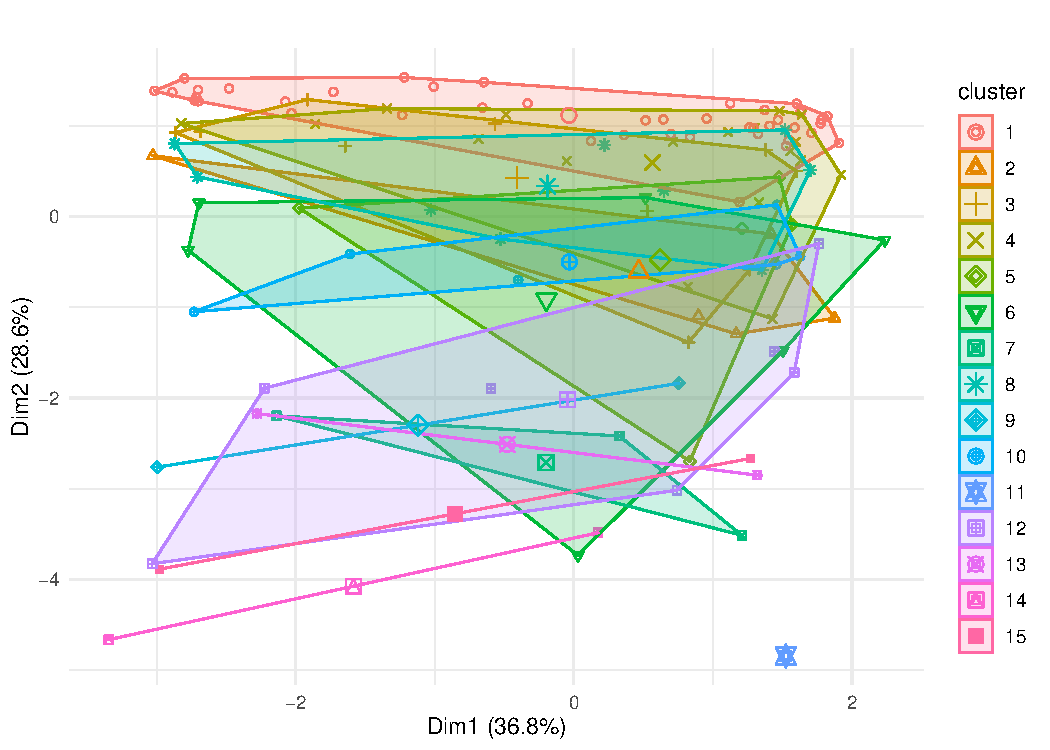
\includegraphics[width=0.5\hsize]{diff-compscatter-15.pdf}
}
\caption{変動値におけるクラスタリング結果の主成分散布図}
\label{diffPseudoFresultPlot}
\end{center}
\end{figure}

変動値におけるクラスタリングにおいて,図 \ref{diffPseudoF}(a) と図 \ref{diffPseudoF}(b) は実測値の場合と同様に単調増加していたが, \ref{diffPseudoF}(c) はクラスタ数 5 にて極大値を取っていた.
主成分分析はより少ない次元数でデータを特徴づけるものであるため,適切なクラスタ数においては主成分散布図上においてもクラスタ間に重なりがなく,クラスタ内の要素は固まっていることが望ましい.図 \ref{diffPseudoFresultPlot}(a) からその傾向を強く見受けることができないが,赤色で表されるクラスタ 1 に属する要素のうち第二主成分が大きなものなどでは他のクラスタと重なりがないため,ある程度は適切なクラスタ数であると考えられる.

\newpage
\subsection{実測値の主成分に対して}
実測値の主成分に対してこれら三つの指標を用いた結果は図 \ref{norm_compPseudoF} となった.
表 \ref{norm_compPseudoFresult} は各指標から定まる最適クラスタ数をまとめたものであり,図 \ref{norm_compPseudoFresultPlot} はそれらの最適クラスタ数でクラスタリングを行ったときの主成分散布図である.
主成分を用いて行ったクラスタリングにおける主成分散布図の第一主成分・第二主成分は,クラスタリングに用いた第一主成分・第二主成分と一致する.

\begin{figure}[tb]
\begin{center}
\subfigure[PseudoF]{
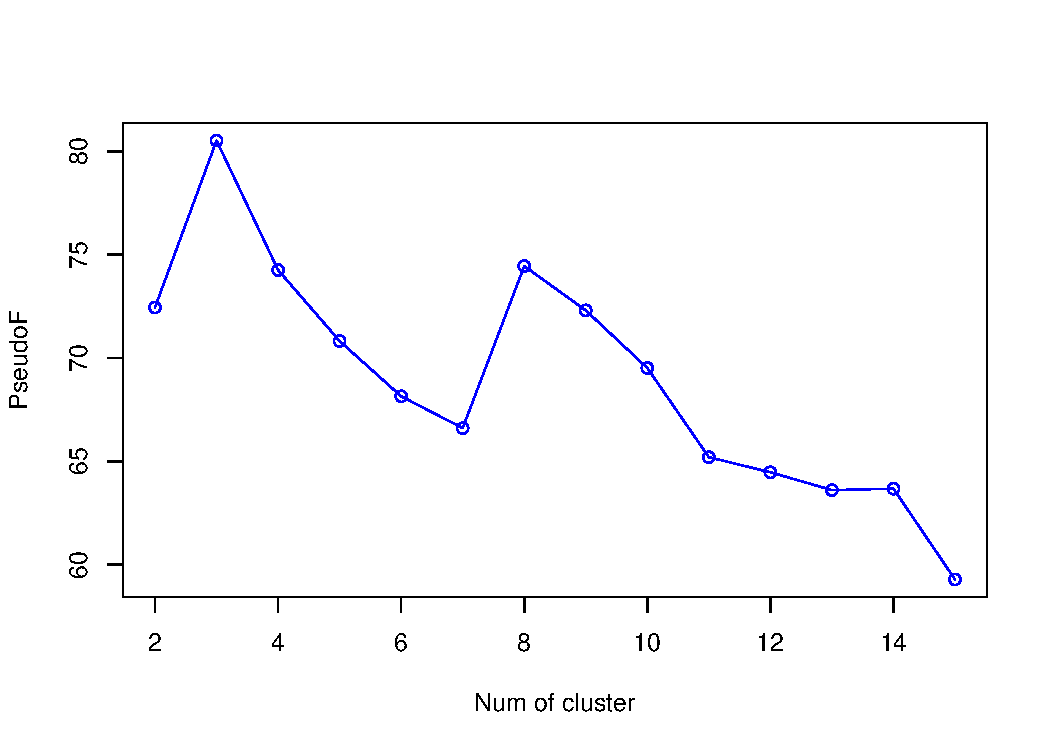
\includegraphics[width=0.33\hsize]{norm_comp-PseudoF.pdf}
}~
\subfigure[PseudoF with Mean]{
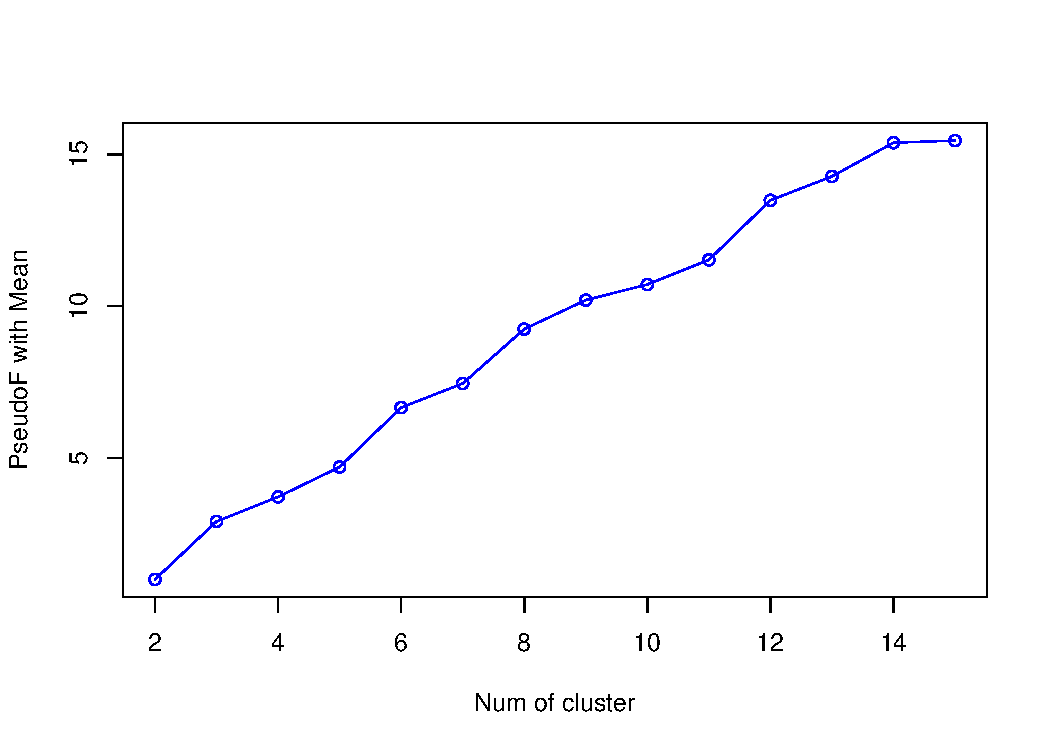
\includegraphics[width=0.33\hsize]{norm_comp-PseudoFwithMean.pdf}
}~
\subfigure[PseudoF with Min]{
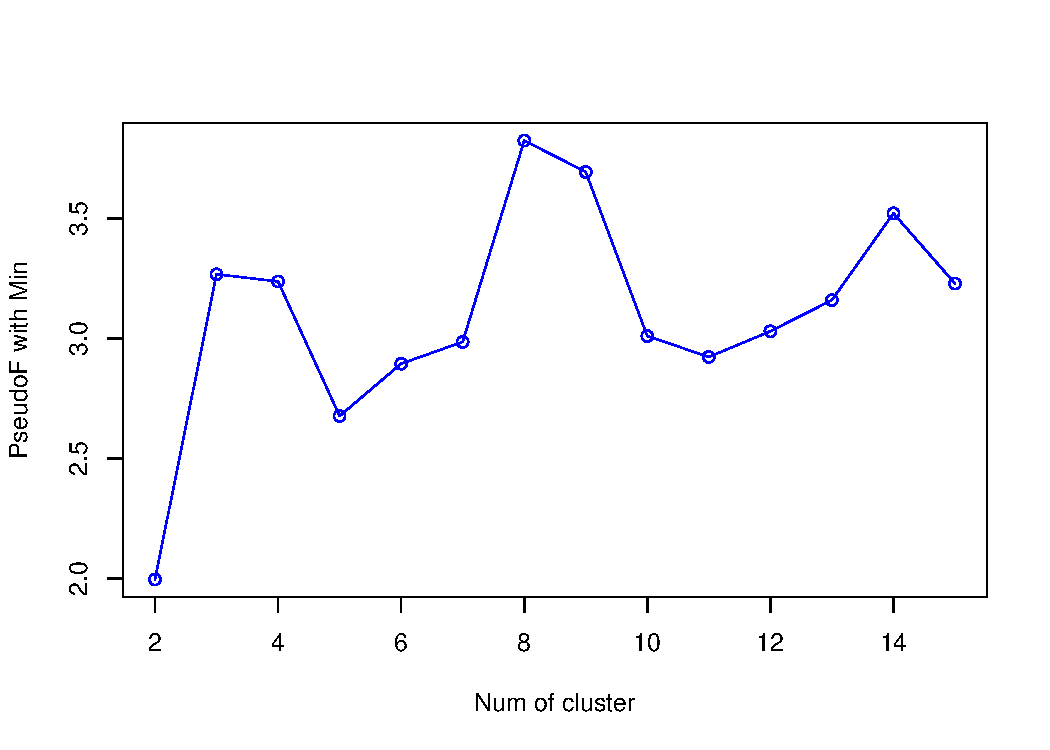
\includegraphics[width=0.33\hsize]{norm_comp-PseudoFwithMin.pdf}
}
\caption{実測値の主成分における最適クラスタ数指標}
\label{norm_compPseudoF}
\end{center}
\end{figure}

\begin{table}[tb]
\centering
\caption{実測値の主成分における最適クラスタ数}
\label{norm_compPseudoFresult}
\begin{tabular}{|c|c|}
\hline
指標&最適クラスタ数\\
\hline
PseudoF&3,8\\
\hline
PseudoF with Mean&15\\
\hline
PseudoF with Min&3,8,14\\
\hline
\end{tabular}
\end{table}

\begin{figure}[tb]
\begin{center}
\subfigure[クラスタ数 3]{
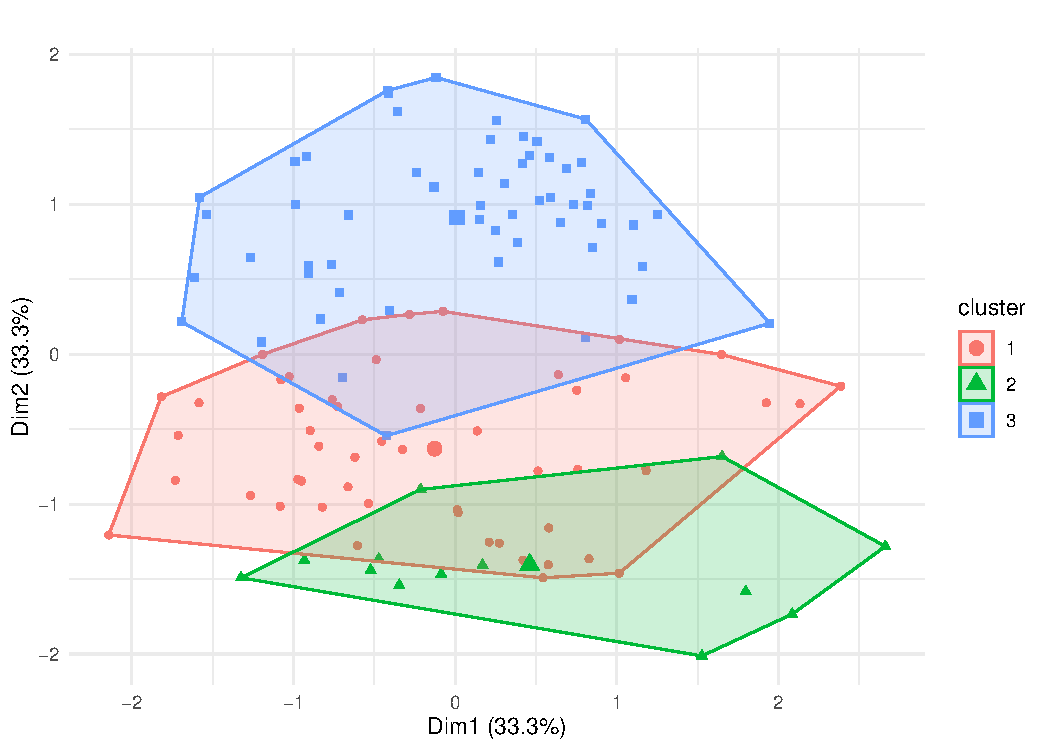
\includegraphics[width=0.5\hsize]{norm_comp-compscatter-3.pdf}
}~
\subfigure[クラスタ数 8]{
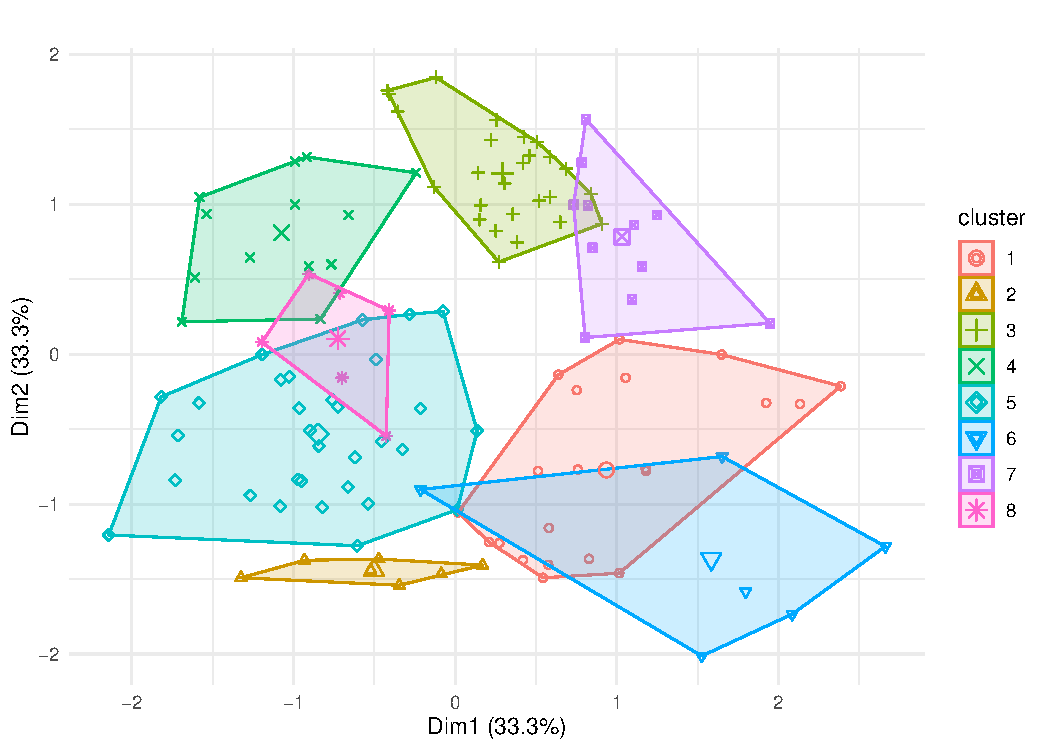
\includegraphics[width=0.5\hsize]{norm_comp-compscatter-8.pdf}
}\\
\subfigure[クラスタ数 14]{
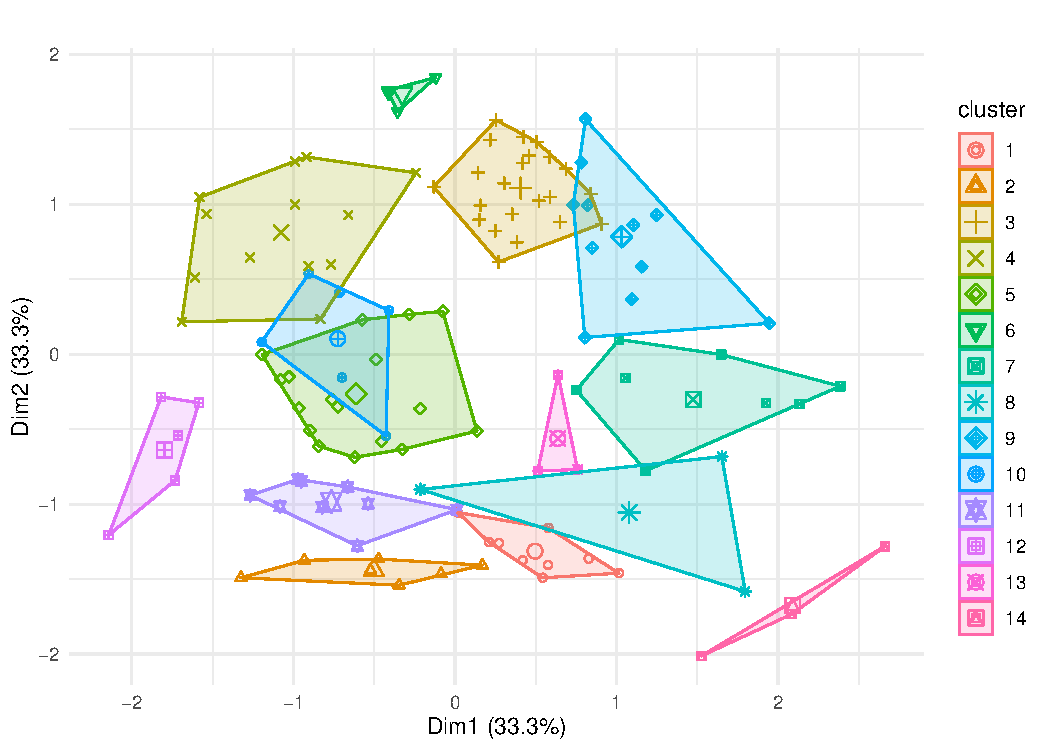
\includegraphics[width=0.5\hsize]{norm_comp-compscatter-14.pdf}
}~
\subfigure[クラスタ数 15]{
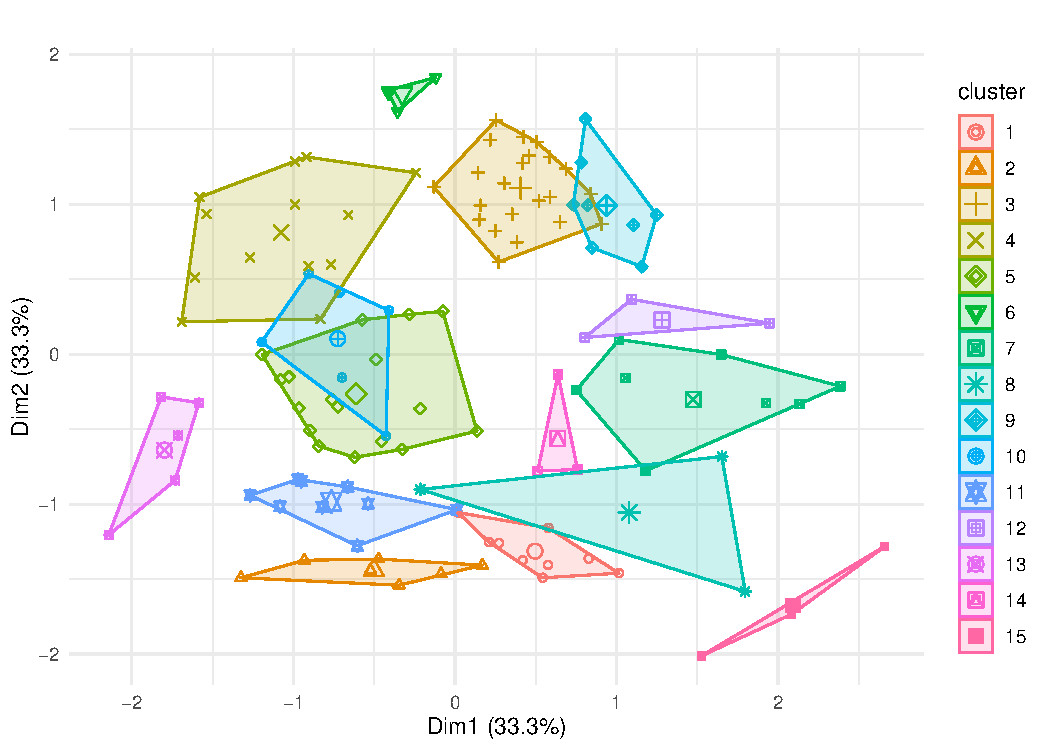
\includegraphics[width=0.5\hsize]{norm_comp-compscatter-15.pdf}
}\\
\caption{実測値の主成分におけるクラスタリング結果の主成分散布図}
\label{norm_compPseudoFresultPlot}
\end{center}
\end{figure}

図 \ref{norm_compPseudoF}(b) は変わらず単調増加しているものの,図  \ref{norm_compPseudoF}(a) においては,クラスタ数 3 と 8 において極大値をとっていた.
したがって,ARMA-GARCH モデルの回帰結果から得られるパラメータを標準化しさらに主成分分析を行った結果得られる主成分を用いることで,クラスタ数が多すぎない範囲で,全データ集合の代表点から各クラスタが散らばった良いクラスタリング結果が得られるようだ.
さらに,図 \ref{norm_compPseudoF}(c) が極大値をとるクラスタ数は図 \ref{norm_compPseudoF}(a) が極大値をとるクラスタ数と一致している.
このことから,主成分を用いたクラスタリングにおいては,指標 PseudoF with Min は,指標 PseudoF を兼ねているようだ.

\newpage
\subsection{変動値の主成分に対して}
変動値の主成分に対してこれら三つの指標を用いた結果は図 \ref{diff_compPseudoF} となった.
表 \ref{diff_compPseudoFresult} は各指標から定まる最適クラスタ数をまとめたものであり,図 \ref{diff_compPseudoFresultPlot} はそれらの最適クラスタ数でクラスタリングを行ったときの主成分散布図である.

\begin{figure}[tb]
\begin{center}
\subfigure[PseudoF]{
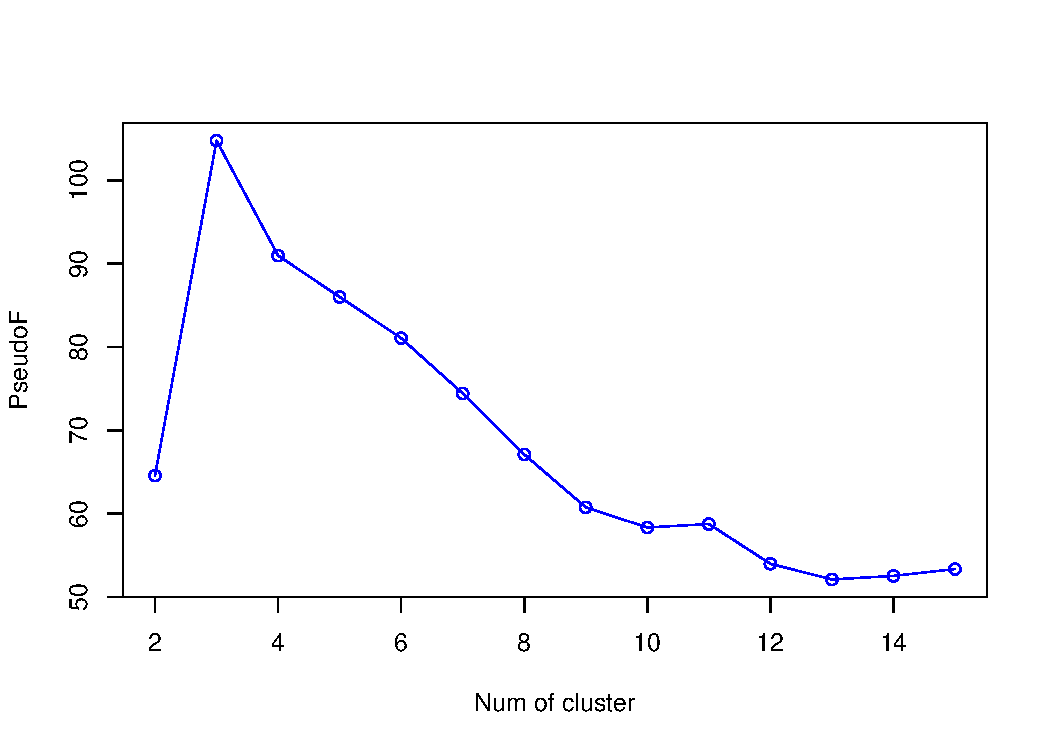
\includegraphics[width=0.33\hsize]{diff_comp-PseudoF.pdf}
}~
\subfigure[PseudoF with Mean]{
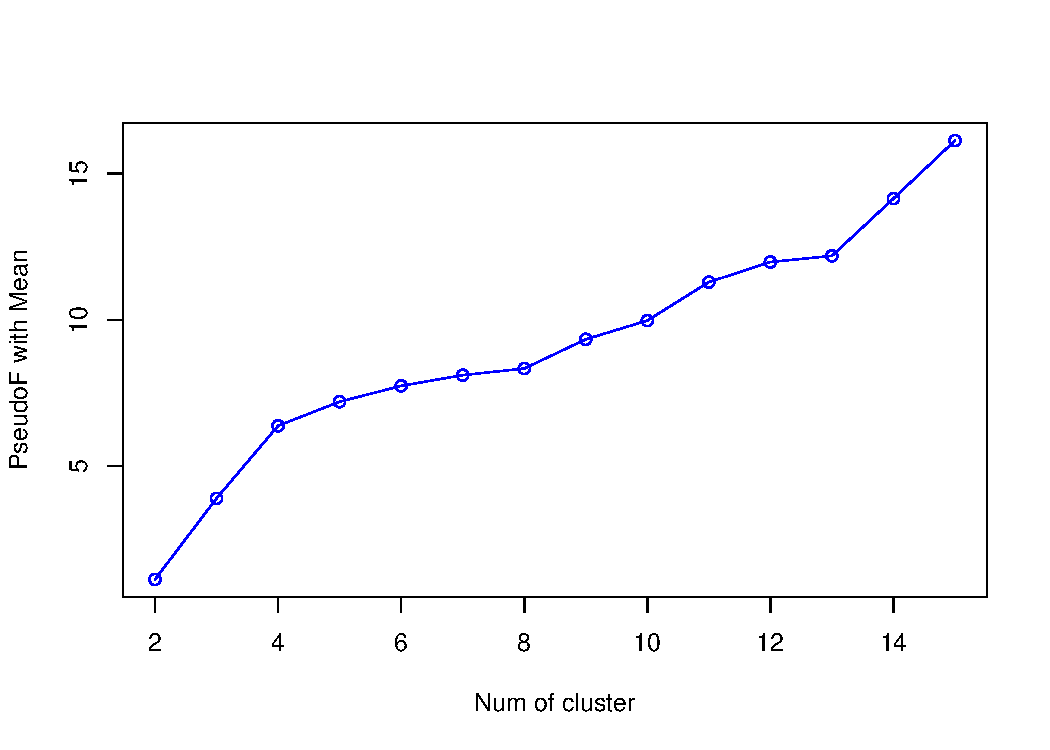
\includegraphics[width=0.33\hsize]{diff_comp-PseudoFwithMean.pdf}
}~
\subfigure[PseudoF with Min]{
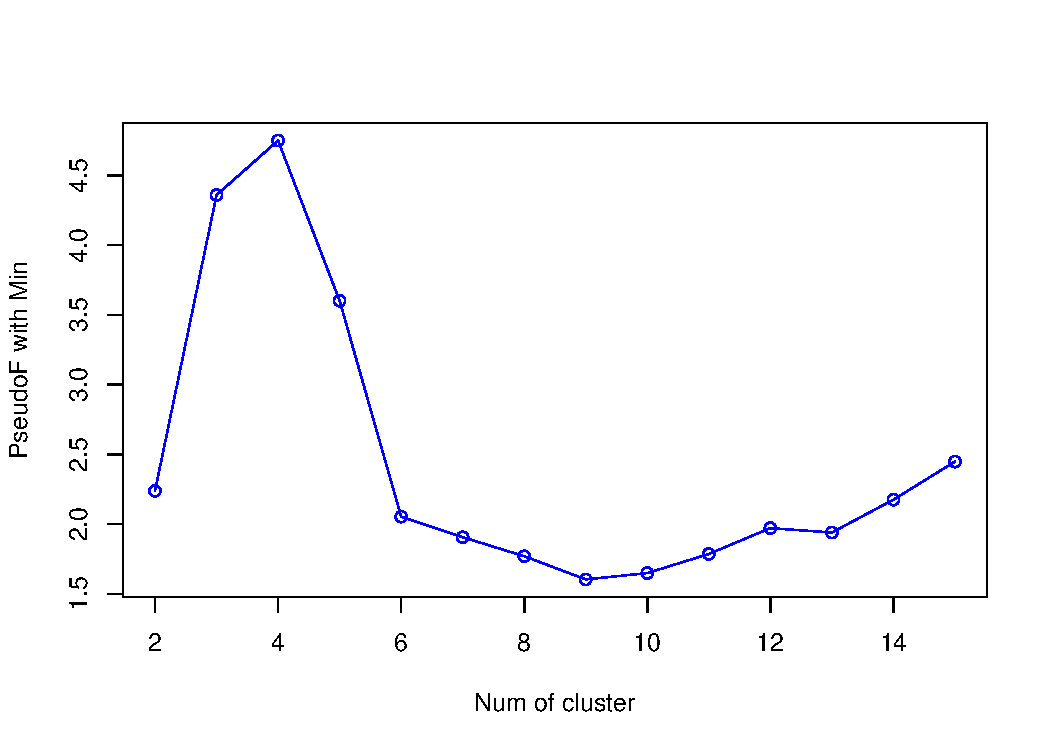
\includegraphics[width=0.33\hsize]{diff_comp-PseudoFwithMin.pdf}
}
\caption{変動値の主成分における最適クラスタ数指標}
\label{diff_compPseudoF}
\end{center}
\end{figure}

\begin{table}[tb]
\centering
\caption{変動値の主成分における最適クラスタ数}
\label{diff_compPseudoFresult}
\begin{tabular}{|c|c|}
\hline
指標&最適クラスタ数\\
\hline
PseudoF&3\\
\hline
PseudoF with Mean&15\\
\hline
PseudoF with Min&4\\
\hline
\end{tabular}
\end{table}

\begin{figure}[tb]
\begin{center}
\subfigure[クラスタ数 3]{
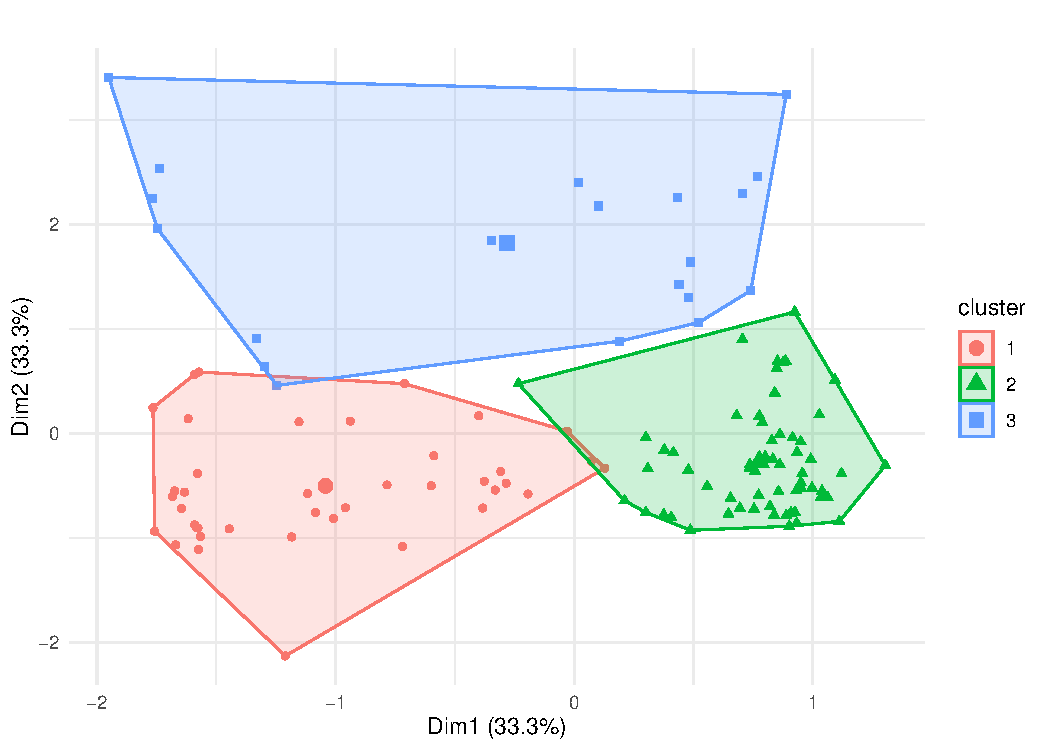
\includegraphics[width=0.5\hsize]{diff_comp-compscatter-3.pdf}
}~
\subfigure[クラスタ数 4]{
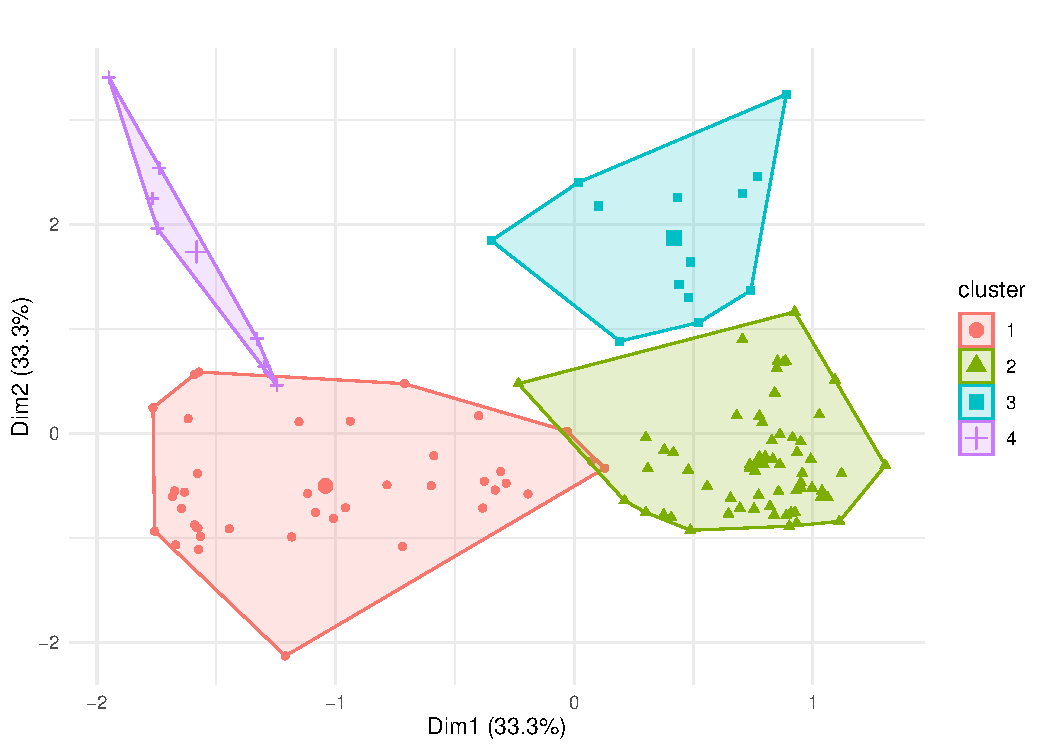
\includegraphics[width=0.5\hsize]{diff_comp-compscatter-4.pdf}
}\\
\subfigure[クラスタ数 15]{
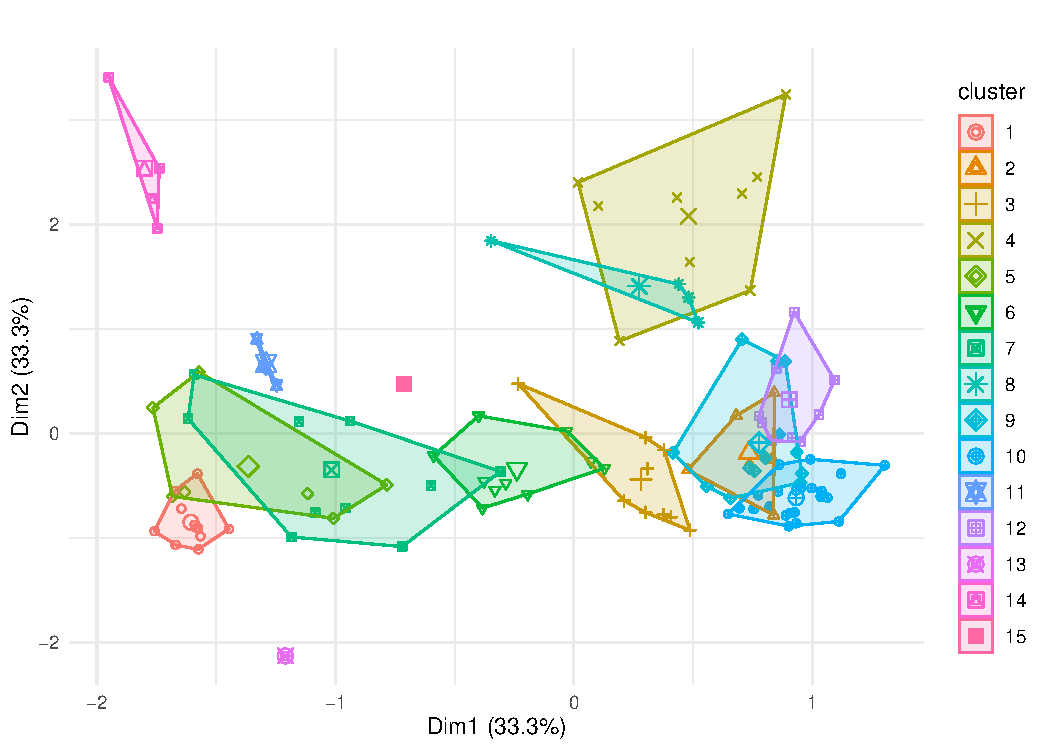
\includegraphics[width=0.5\hsize]{diff_comp-compscatter-15.pdf}
}
\caption{変動値の主成分におけるクラスタリング結果の主成分散布図}
\label{diff_compPseudoFresultPlot}
\end{center}
\end{figure}

実測値の主成分に対してのものと同様に,図 \ref{diff_compPseudoF}(b) は単調増加しており,図 \ref{diff_compPseudoF}(a) と図 \ref{diff_compPseudoF}(c) はほぼ同じクラスタ数の時に極大値をとっていた.
したがって,指標としては PseudoF か PseudoF with Min が適切と考える.

\subsection{結論}
クラスタリングは,標準化後の主成分を用いて行う方が良いだろう.
また,クラスタ数を定める指標としては PseudoF か PseudoF with Min が良いだろう.
ただ,PseudoF with Min では,変動値においても極大値を見いだせており,PseudoF のように値が単調に増加し最適クラスタ数が見つからないことがなかったため,PseudoF with Min がより適切だと考える.

\newpage
\section{クラスタリング結果}
クラスタリング結果を,(a)横軸をクラスタ番号とし計測した時間帯ごとに色分けした積み上げ棒グラフ,(b) 横軸をクラスタ番号とし計測した曜日ごとに色分けした積み上げ棒グラフ,(c)横軸を計測した曜日と時間帯とし属するクラスタ番号ごとに色分けした積み上げ棒グラフ,を示す.
縦軸は全て割合としており,各棒の上部にその要素数を示している.
\subsection{実測値の主成分に対して}
1.3 章よりクラスタ数を 8 とした場合を図 \ref{norm} に示す.
\begin{figure}[tb]
\begin{center}
\subfigure[時間帯ごとに属するクラスタ]{
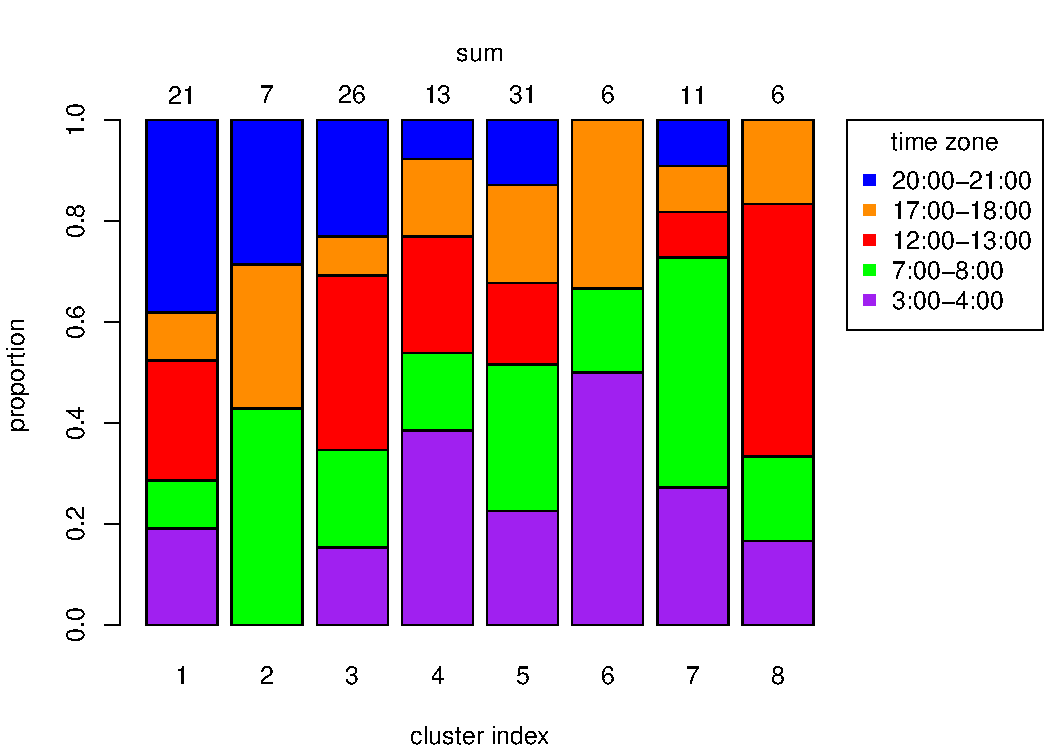
\includegraphics[width=0.5\hsize]{norm_comp-eucl-ward-8-timezone.pdf}
}~
\subfigure[曜日ごとに属するクラスタ]{
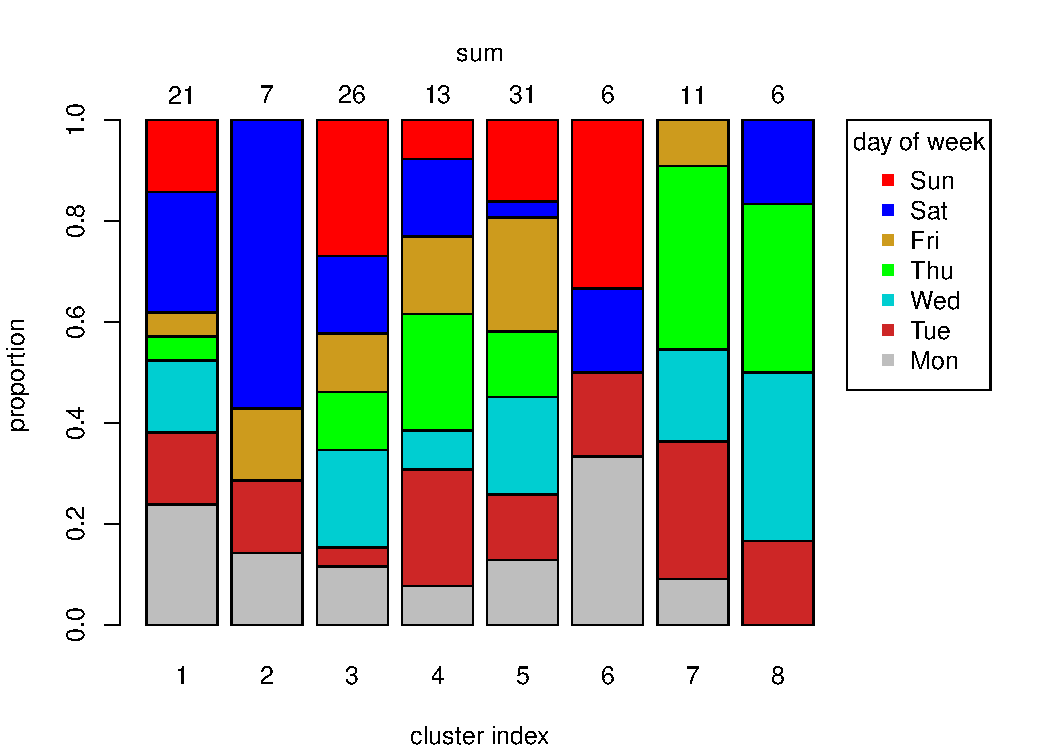
\includegraphics[width=0.5\hsize]{norm_comp-eucl-ward-8-day.pdf}
}\\
\subfigure[各時間帯と曜日が属するクラスタ]{
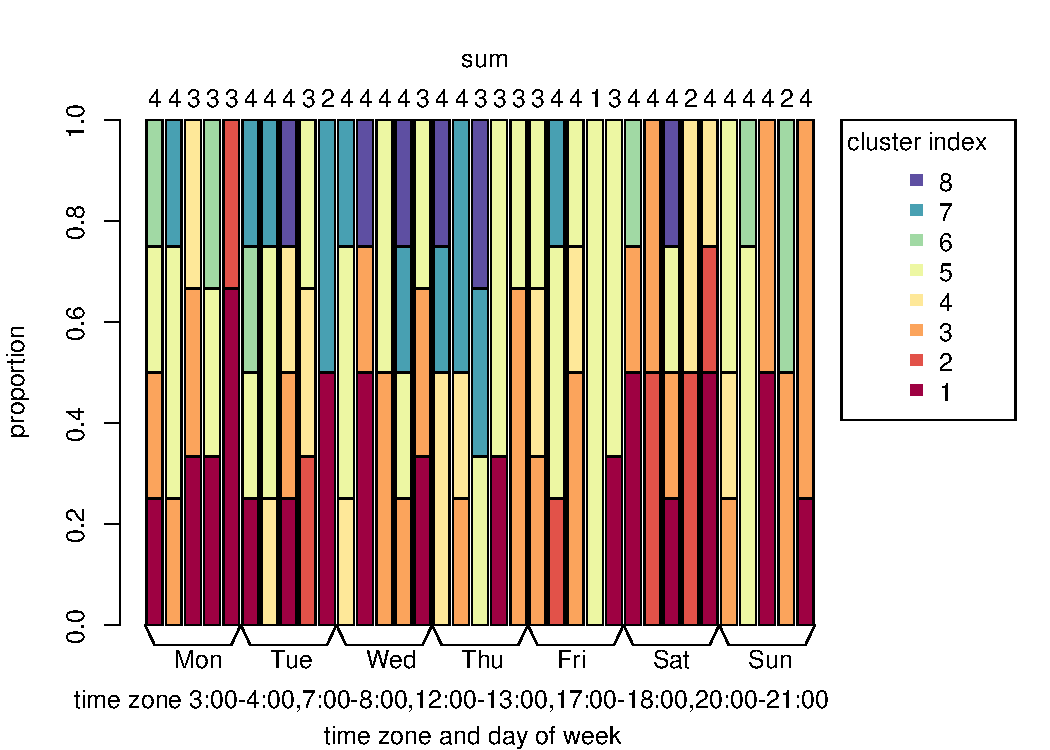
\includegraphics[width=0.5\hsize]{norm_comp-eucl-ward-8-timezone-day.pdf}
}
\caption{実測値の主成分をもとにクラスタ数 8 で行ったクラスタリング結果}
\label{norm}
\end{center}
\end{figure}

図 \ref{norm}(a) のクラスタ番号 1 には 20:00 - 21:00 に計測したデータが多く属しており,図 \ref{norm}(c) より全ての曜日の 20:00 - 21:00 の計測データのうち少なくとも一つはクラスタ番号 1 に属していたため,このクラスタには 20:00 - 21:00 の計測データが属しやすいといえそうだ.
ただ,他のクラスタ番号において全曜日の同一時間帯に計測されたデータが属するクラスタは見受けられなかった.

図 \ref{norm}(a) のクラスタ番号 1 と 3 は,利用者が多いと考えられる 12:00 - 13:00,17:00-18:00,20:00-21:00 の計測データの割合が多い.
さらに,図 \ref{norm}(b) のクラスタ番号 1 と 3 は,利用者が多いと考えられる土曜日と日曜日の割合が多い.
これは図 \ref{norm}(c) からも読み取れる.
したがって,クラスタ番号 1 と 3 には,利用者が多い状況で計測されたデータが属しやすい傾向があるのではないか.

逆に図 \ref{norm}(a) のクラスタ番号 7 は,利用者が少ないと考えられる 3:00 - 4:00,7:00 - 8:00 の計測データが多く,図 \ref{norm}(b) のクラスタ番号 7 には利用者が多いと考えられる土曜日と日曜日に計測されたデータは属していなかった.
したがって,クラスタ番号 7 には,利用者が多くない状況で計測されたデータが属しやすい傾向があるのではないか.

要素数が少ないクラスタであるクラスタ番号 2 と 6 と 8 のそれぞれにおいて,同一時間帯や同一曜日,または同一の時間帯と曜日のデータが,この他のデータ集合から外れたクラスタに属する傾向があるかを調べたが,この結果からはそのような傾向は見受けられなかった.

\newpage
\subsection{変動値の主成分に対して}
1.4 章よりクラスタ数を 4 とした場合を図 \ref{diff} に示す.
\begin{figure}[tb]
\begin{center}
\subfigure[時間帯ごとに属するクラスタ]{
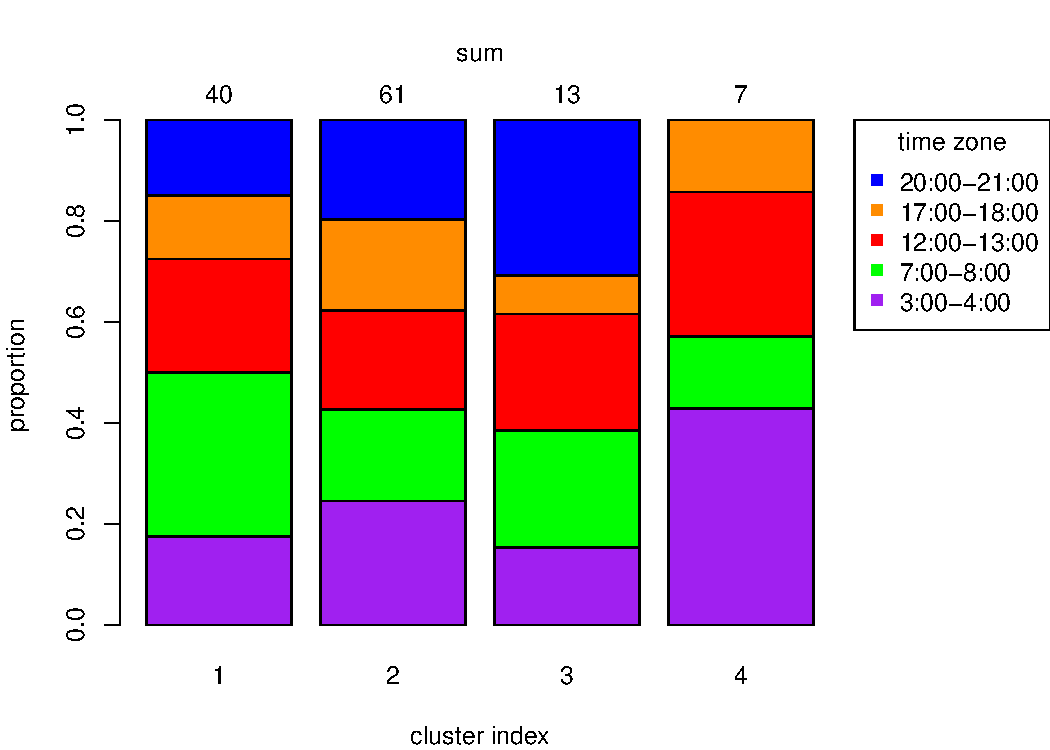
\includegraphics[width=0.5\hsize]{diff_comp-eucl-ward-4-timezone.pdf}
}~
\subfigure[曜日ごとに属するクラスタ]{
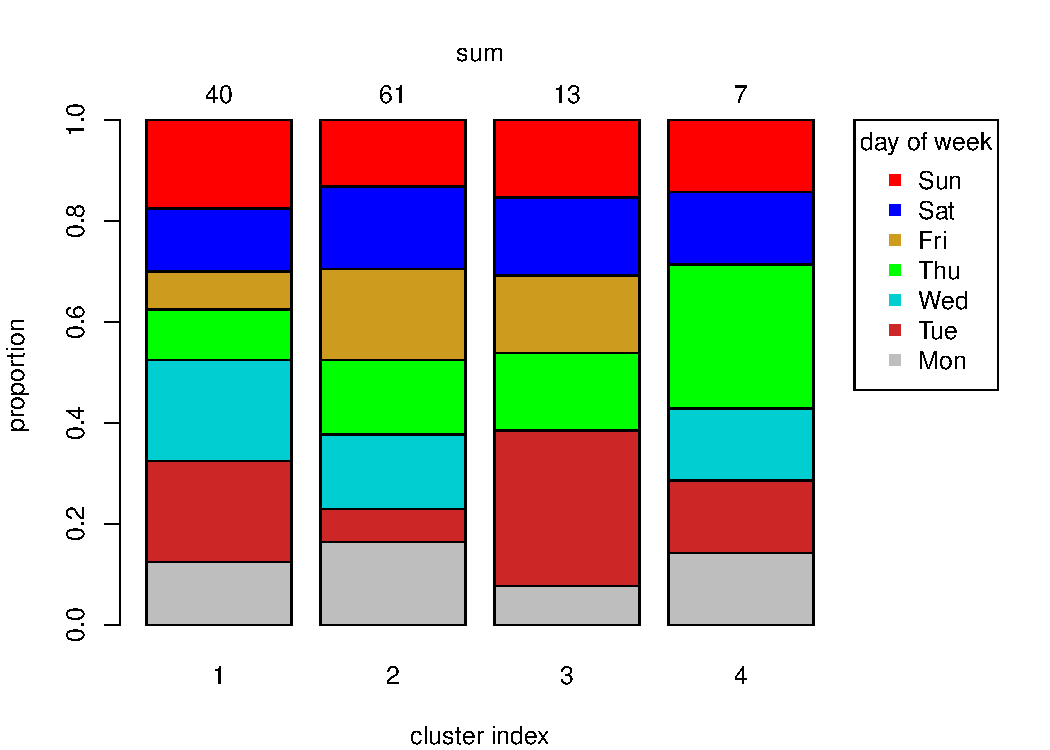
\includegraphics[width=0.5\hsize]{diff_comp-eucl-ward-4-day.pdf}
}\\
\subfigure[各時間帯と曜日が属するクラスタ]{
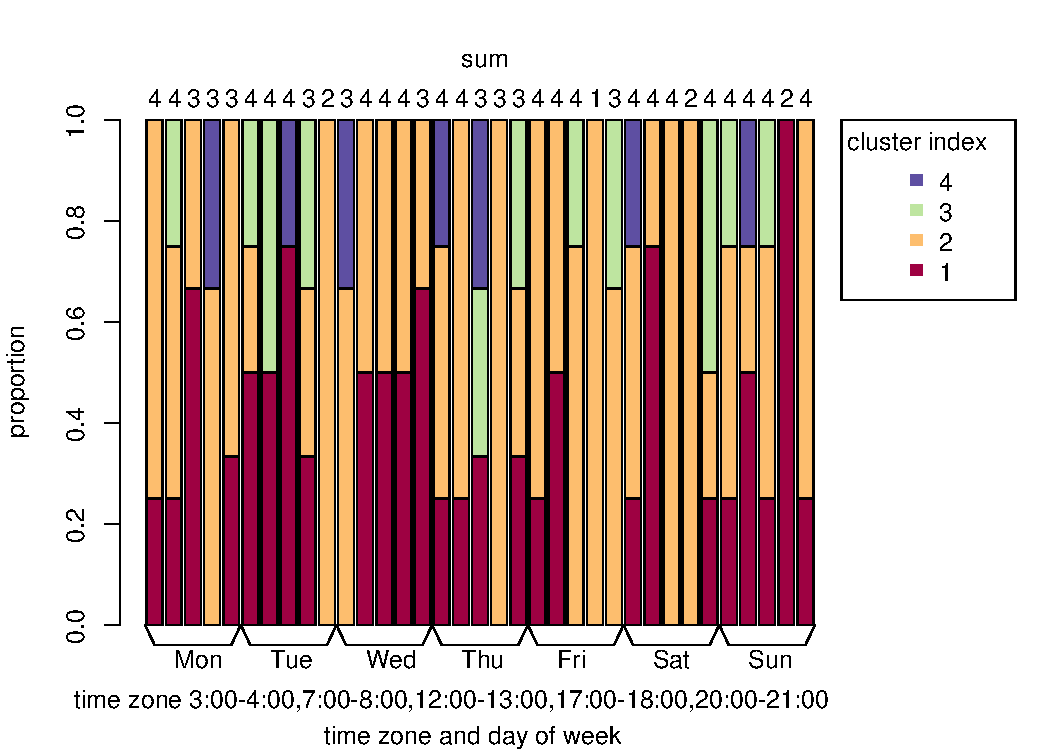
\includegraphics[width=0.5\hsize]{diff_comp-eucl-ward-4-timezone-day.pdf}
}
\caption{変動値の主成分をもとにクラスタ数 4 で行ったクラスタリング結果}
\label{diff}
\end{center}
\end{figure}

変動値の主成分を用いたクラスタリングでは,最適クラスタ数が 4 と少なく,さらに多くのデータが図 \ref{diff}(a) のクラスタ番号 1 か 2 に属していた.
図 \ref{diff}(c) からはどの曜日のどの時間帯においてもまんべんなくクラスタ番号 1 か 2 に属していることが見て取れる.
またこれらのクラスタから外れた要素数の少ないクラスタのクラスタ番号 3 か 4 に属するデータには,計測時間帯や曜日に共通性は見て取れない.
したがって,変動値はおおよそクラスタ番号 1 か 2 で代表され,そこから外れる場合もあるがそこに共通性はなさそうだ.
よって,変動値の主成分を用いたクラスタリングを用いた異常検知方法としては,現場の無線機器で一定の時間幅の取得データをもとにクラスタリングを行い,要素数の多いクラスタから外れ続けた場合に異常とみなすことなどが考えられる.

\newpage
\section{まとめと今後の課題}
実測値の主成分を用いたクラスタリング結果においては,曜日や時間帯に応じた傾向が存在する可能性が見受けられた.
そのため障害検知手法としては,例えば,前もって行ったクラスタリング結果において形成された曜日や時間帯ごとの傾向を持つクラスタの代表点を,その曜日や時間帯における ARMA-GARCH モデルのパラメータのテンプレートとし,それを用いて行った応答遅延の予測値から実測値が大きく外れ続けた場合に異常を検知することが考えられる.
または,現場の無線機器で逐次クラスタリングを行った結果が,その計測時における曜日や時間帯の傾向を持つ代表点のクラスタに属さなかった場合に異常を検知することも考えられる.
しかし,今回得られたクラスタリング結果においては,曜日や時間帯に応じた傾向を顕著に見て取ることができなかった.
これには様々な原因が考えられるがそのうちの一つとして,単発的に発生する応答遅延によりモデルの回帰精度が悪くなっていることが考えられる.
また,時系列モデルの回帰において,スパイク的な応答遅延を予測することができないため,異常に大きな遅延が発生したり,頻繁に大きな遅延が発生したりする異常は検知できないと思われる.
そのため,実用的な異常検知には,単発的な応答遅延の発生頻度やそのスパイク性を表す別の手法と組み合わせることが必要であろう.
\end{document}